\subsubsection{Examples of Linear Image Filters}\label{sec:examples-of-linear-image-filters}

Now we make the abstract formula from the previous section concrete. Recall:
\begin{equation*}
    T[I](r,c) = \sum_{(u,v) \in U} w(u,v) I(r+u, c+v)
\end{equation*}
The operation is always the same:
\begin{equation*}
    \text{local patch} \to \text{weighted sum} \to \text{one output pixel}
\end{equation*}
What changes is only the filter $\mathbf{w}$. So \hl{different filter weights produce different image transformations.}

\highspace
\begin{flushleft}
    \textcolor{Green3}{\faIcon{book} \textbf{Identity filter}}
\end{flushleft}
The \definition{Identity Filter} is the simplest possible filter. It has a single non-zero weight in the center of the filter, and all other weights are zero. The effect of this filter is to leave the image unchanged.
\begin{equation}
    \mathbf{w}_{\text{id}} = \begin{bmatrix}
        0 & 0 & 0 \\
        0 & 1 & 0 \\
        0 & 0 & 0
    \end{bmatrix}
\end{equation}
At spatial position $(r,c)$, the output pixel is simply the input pixel at that position:
\begin{equation*}
    T[I](r,c) = 0 \cdot I(r-1,c-1) + \cdots + 1 \cdot I(r,c) + \cdots + 0 \cdot I(r+1,c+1) = I(r,c)
\end{equation*}
So the output image is identical to the input image: $T[I] = I$.

\highspace
% Averaging filter
\begin{flushleft}
    \textcolor{Green3}{\faIcon{book} \textbf{Averaging filter}}
\end{flushleft}
The \definition{Averaging Filter} is a simple filter that computes the \textbf{average of the pixel values in a local neighborhood}. It has \hl{equal weights for all pixels in the filter}, and the \hl{sum of the weights is 1.} The effect of this filter is to \textbf{smooth the image}, reducing noise and detail.
\begin{equation}
    \mathbf{w}_{\text{avg}} = \frac{1}{9} \begin{bmatrix}
        1 & 1 & 1 \\
        1 & 1 & 1 \\
        1 & 1 & 1
    \end{bmatrix}
\end{equation}
At every position, the output pixel is:
\begin{equation*}
    T[I](r,c) = \frac{1}{9} \sum_{u=-1}^{1} \sum_{v=-1}^{1} I(r+u, c+v)
\end{equation*}
This is simply the average of the 9 pixels in the $3 \times 3$ neighborhood centered at $(r,c)$. For example, suppose the local patch of the image is:
\begin{equation*}
    \begin{bmatrix}
        10 & 10 & 10 \\
        10 & 100 & 10 \\
        10 & 10 & 10
    \end{bmatrix}
\end{equation*}
The central pixel is much brighter than its neighbors. The filtered value becomes:
\begin{equation*}
    T[I](r,c) = \frac{1}{9} (10 + 10 + 10 + 10 + 100 + 10 + 10 + 10 + 10) = \frac{180}{9} = 20
\end{equation*}
So the central value changes from 100 to 20, which is much closer to the values of its neighbors.

\highspace
For example, consider the following Lena image. The left image is the original, and the right image is the result of applying the $3 \times 3$ averaging filter to every pixel in the original image. The \hl{filtered image appears slightly softer because each pixel is replaced by an average of itself and its neighbours.} Fine variations are reduced, while slowly varying regions remain similar.

\begin{figure}[!htp]
    \centering

    \begin{subfigure}[t]{0.49\textwidth}
        \centering
        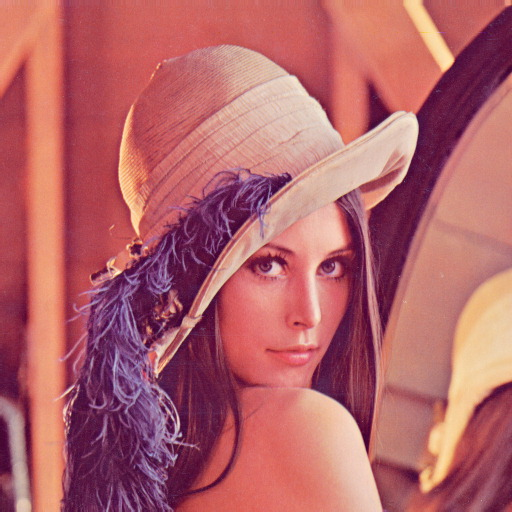
\includegraphics[width=\linewidth]{img/cnn/lena.jpg}
        \caption{Original image}
    \end{subfigure}
    \hfill
    \begin{subfigure}[t]{0.49\textwidth}
        \centering
        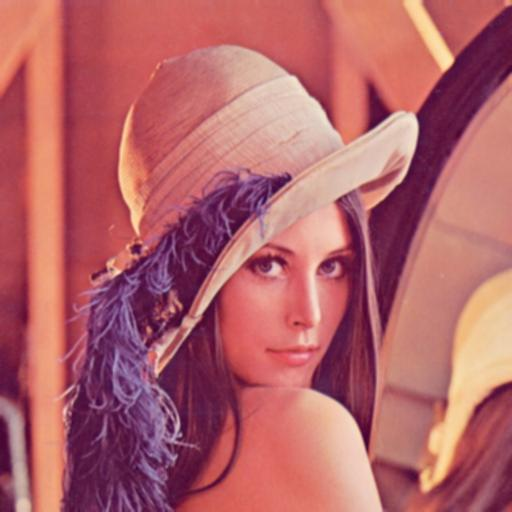
\includegraphics[width=\linewidth]{img/cnn/lena_average_3x3.jpg}
        \caption{After a $3\times3$ averaging filter}
    \end{subfigure}

    \caption{Effect of a $3\times3$ averaging filter. Each output pixel is the average of its $3\times3$ neighbourhood, producing a smoother image and reducing fine details.}
    \label{fig:lena-average}
\end{figure}

\noindent
\textcolor{Green3}{\faIcon{question-circle} \textbf{What happens at an edge?}} Suppose we look at the pixel exactly on the white side. Its neighbourhood is:
\begin{equation*}
    \begin{bmatrix}
        0 & 0 & 255 \\
        0 & 255 & 255 \\
        0 & 255 & 255
    \end{bmatrix}
\end{equation*}
Notice that some neighbours are black, while others are white. If we apply the averaging filter, the filter computes the average of these 9 values:
\begin{equation*}
    T[I](r,c) = \frac{1}{9} (0 + 0 + 255 + 0 + 255 + 255 + 0 + 255 + 255) = \frac{1530}{9} = 170
\end{equation*}
So the central pixel value changes from 255 to 170, which is a gray value. We do not get a sudden jump from black to white, but rather a \textbf{smooth transition}.

\highspace
\textcolor{Green3}{\faIcon{question-circle} \textbf{What happens to noise?}} Imagine a completely gray wall. Every pixel should be $100$. But one sensor measurement is wrong and the center is much brighter than it should be:
\begin{equation*}
    \begin{bmatrix}
        100 & 100 & 100 \\
        100 & 180 & 100 \\
        100 & 100 & 100
    \end{bmatrix}
\end{equation*}
Applying the averaging filter, the central pixel value becomes:
\begin{equation*}
    T[I](r,c) = \frac{1}{9} (100 + 100 + 100 + 100 + 180 + 100 + 100 + 100 + 100) = \frac{980}{9} = 108.9 \approx 109
\end{equation*}
Instead of being 180, the central pixel is now 109, which is much closer to the expected value of 100. The averaging filter has \textbf{reduced the effect of noise}.

\highspace
In summary, every averaging filter performs the same operation: average nearby pixels. Therefore:
\begin{itemize}
    \item If neighbouring differences are caused by \textbf{noise}, averaging is beneficial;
    \item If neighbouring differences correspond to \textbf{real image details} (edges, textures, thin structures), averaging destroys part of that information.
\end{itemize}

\highspace
\textcolor{Green3}{\faIcon{question-circle} \textbf{What happens if we use a larger averaging filter?}} A larger averaging filter will include more pixels in the average, which will \textbf{increase the smoothing effect}. For example, a $5 \times 5$ averaging filter will average over 25 pixels instead of 9:
\begin{equation*}
    \mathbf{w}_{\text{avg},5} = \frac{1}{25} \begin{bmatrix}
        1 & 1 & 1 & 1 & 1 \\
        1 & 1 & 1 & 1 & 1 \\
        1 & 1 & 1 & 1 & 1 \\
        1 & 1 & 1 & 1 & 1 \\
        1 & 1 & 1 & 1 & 1
    \end{bmatrix}
\end{equation*}
Now each output value is the average of $25$ nearby pixels:
\begin{equation*}
    T[I](r,c) = \frac{1}{25} \sum_{u=-2}^{2} \sum_{v=-2}^{2} I(r+u, c+v)
\end{equation*}
In general, for an $m \times m$ averaging filter, the normalized coefficients are:
\begin{equation*}
    w(u,v) = \frac{1}{m^2}
\end{equation*}
Thus, the output pixel is:
\begin{equation*}
    \mathbf{w}_{\text{avg},m} = \frac{1}{m^2} \begin{bmatrix}
        1 & 1 & \cdots & 1 \\
        1 & 1 & \cdots & 1 \\
        \vdots & \vdots & \ddots & \vdots \\
        1 & 1 & \cdots & 1
    \end{bmatrix}
\end{equation*}
So increasing the kernel size $m$ \textbf{increases the smoothing effect} without systematically changing constant-region brightness (i.e., the average of a constant region remains the same). However, it also increases the \textbf{risk of losing important image details} because the filter averages over a larger area, which can blur edges and textures.

\begin{figure}[!htp]
    \centering

    \begin{subfigure}[t]{0.49\textwidth}
        \centering
        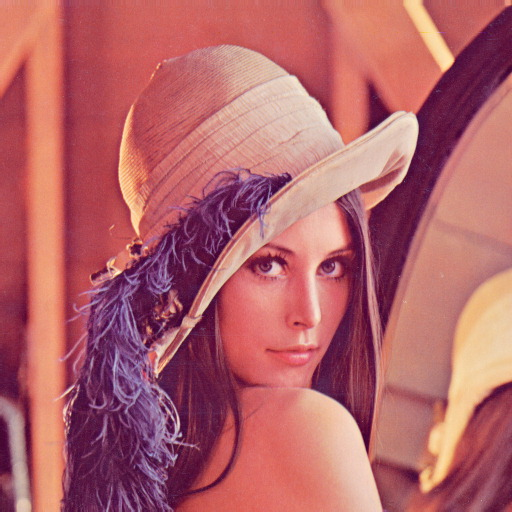
\includegraphics[width=\linewidth]{img/cnn/lena.jpg}
        \caption{Original image}
    \end{subfigure}
    \hfill
    \begin{subfigure}[t]{0.49\textwidth}
        \centering
        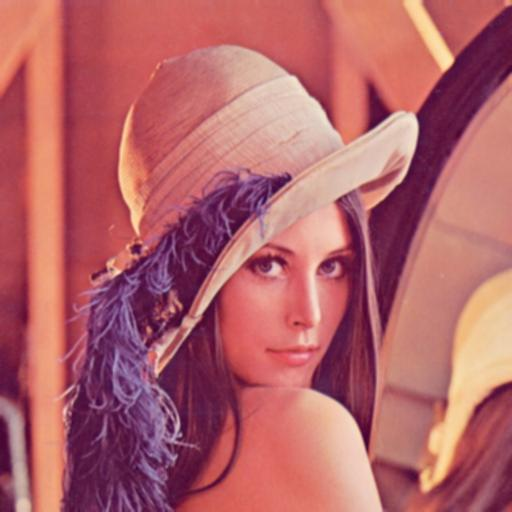
\includegraphics[width=\linewidth]{img/cnn/lena_average_3x3.jpg}
        \caption{After a $3\times3$ averaging filter}
    \end{subfigure}

    \vspace{0.3cm}

    \begin{subfigure}[t]{0.49\textwidth}
        \centering
        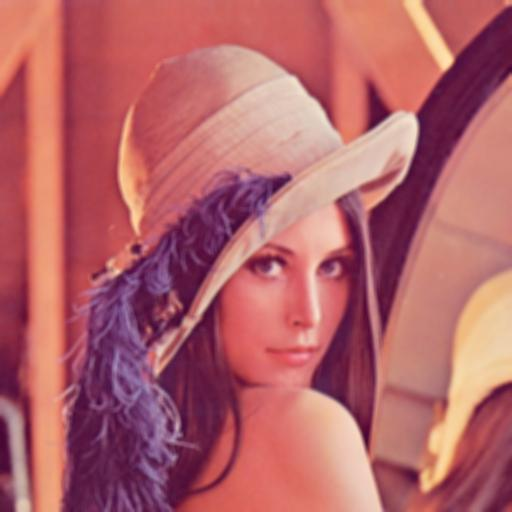
\includegraphics[width=\linewidth]{img/cnn/lena_average_5x5.jpg}
        \caption{After a $5\times5$ averaging filter}
    \end{subfigure}
    \hfill
    \begin{subfigure}[t]{0.49\textwidth}
        \centering
        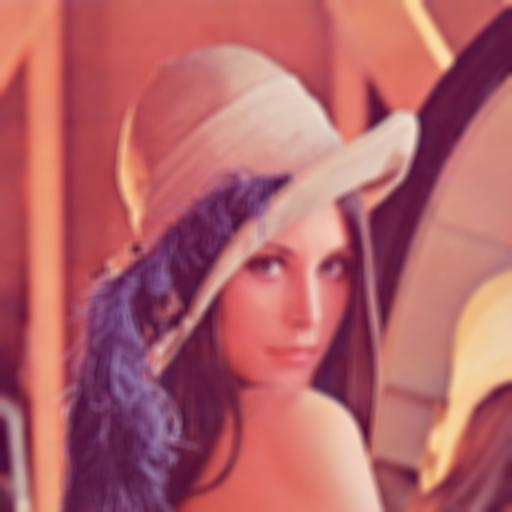
\includegraphics[width=\linewidth]{img/cnn/lena_average_9x9.jpg}
        \caption{After a $9\times9$ averaging filter}
    \end{subfigure}

    \caption{Effect of increasing the averaging filter size. As the filter size increases, the image becomes progressively smoother and more blurred, losing fine details and textures.}
    \label{fig:lena-average-9x9}
\end{figure}

\highspace
\begin{flushleft}
    \textcolor{Green3}{\faIcon{book} \textbf{Motion Blur filter}}
\end{flushleft}
The \definition{Motion Blur Filter} is a filter that simulates the effect of motion blur in an image. It has non-zero weights along a diagonal line, and all other weights are zero. The effect of this filter is to \textbf{blur the image in a specific direction}, simulating the effect of camera motion during exposure.
\begin{equation}
    \mathbf{w}_{\text{motion}} = \frac{1}{L} \begin{bmatrix}
        1 & 0 & 0 & \cdots & 0 \\
        0 & 1 & 0 & \cdots & 0 \\
        0 & 0 & 1 & \cdots & 0 \\
        \vdots & \vdots & \vdots & \ddots & \vdots \\
        0 & 0 & 0 & \cdots & 1
    \end{bmatrix}
\end{equation}
Where:
\begin{itemize}
    \item $L$ is the \textbf{length of the motion blur} (number of pixels to average over, called also blur length);
    \item The \textbf{main diagonal} determines the \textbf{direction} of the blur (e.g., top-left to bottom-right, or top-right to bottom-left);
    \item The factor $\frac{1}{L}$ normalizes the kernel so that its coefficients sum to 1, preserving the average brightness.
\end{itemize}
The diagonal filter averages the pixel values along the diagonal direction, thus the details are spread along that diagonal, structures become blurred preferentially in that direction, and the effect is directional rather than isotropic like the averaging filter.

\highspace
Mathematically, we can express the motion blur as:
\begin{equation*}
    I_\text{blurred} = I_{\text{sharp}} * \mathbf{w}_{\text{motion}}
\end{equation*}
Where $I_{\text{sharp}}$ is the original image, $I_\text{blurred}$ is the resulting blurred image, and $*$ denotes correlation (or convolution) with the motion blur kernel $\mathbf{w}_{\text{motion}}$.

\begin{figure}[!htp]
    \centering

    \begin{subfigure}[t]{0.49\textwidth}
        \centering
        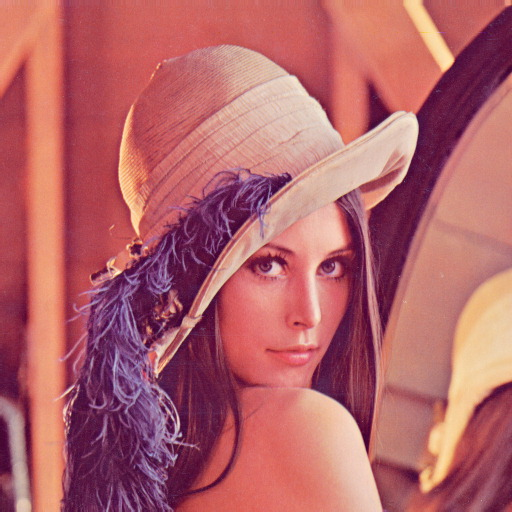
\includegraphics[width=\linewidth]{img/cnn/lena.jpg}
        \caption{Original Image}
    \end{subfigure}
    \hfill
    \begin{subfigure}[t]{0.49\textwidth}
        \centering
        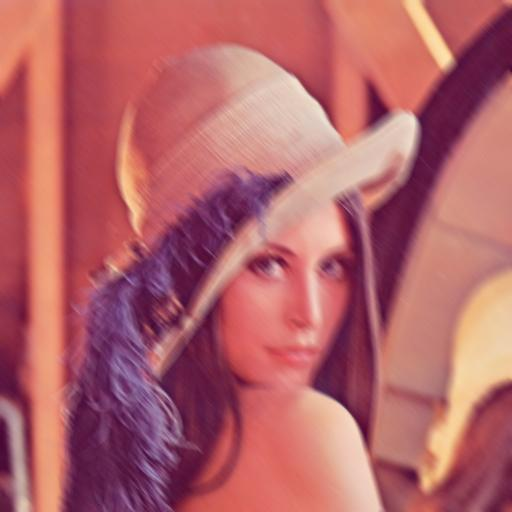
\includegraphics[width=\linewidth]{img/cnn/lena_blur_9x9_45deg.jpg}
        \caption{After a $9\times9$ motion blur filter at 45 degrees (main diagonal)}
    \end{subfigure}
    \vspace{0.3cm}
    \begin{subfigure}[t]{0.49\textwidth}
        \centering
        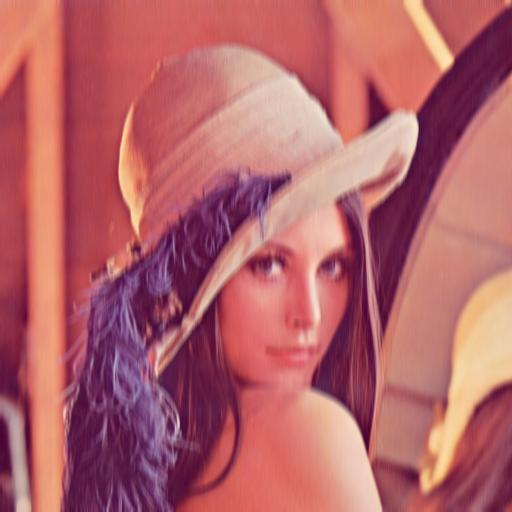
\includegraphics[width=\linewidth]{img/cnn/lena_blur_9x9_90deg.jpg}
        \caption{After a $9\times9$ motion blur filter at 90 degrees (vertical)}
    \end{subfigure}
    \hfill
    \begin{subfigure}[t]{0.49\textwidth}
        \centering
        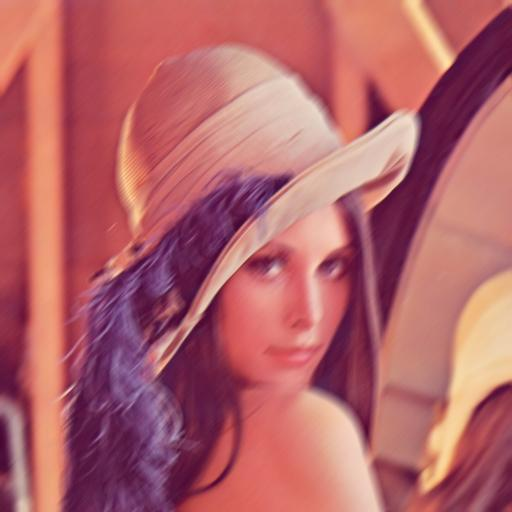
\includegraphics[width=\linewidth]{img/cnn/lena_blur_9x9_135deg.jpg}
        \caption{After a $9\times9$ motion blur filter at 135 degrees (anti-diagonal)}
    \end{subfigure}

    \caption{Effect of a $9\times9$ motion blur filter. The image appears blurred along the diagonal direction, simulating the effect of camera motion during exposure.}
    \label{fig:lena-motion-blur-9x9}
\end{figure}

\begin{figure}[!htp]
    \centering

    \begin{subfigure}[t]{0.49\textwidth}
        \centering
        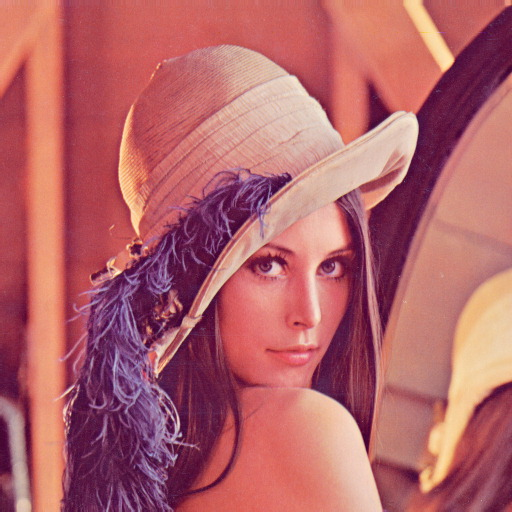
\includegraphics[width=\linewidth]{img/cnn/lena.jpg}
        \caption{Original Image}
    \end{subfigure}
    \hfill
    \begin{subfigure}[t]{0.49\textwidth}
        \centering
        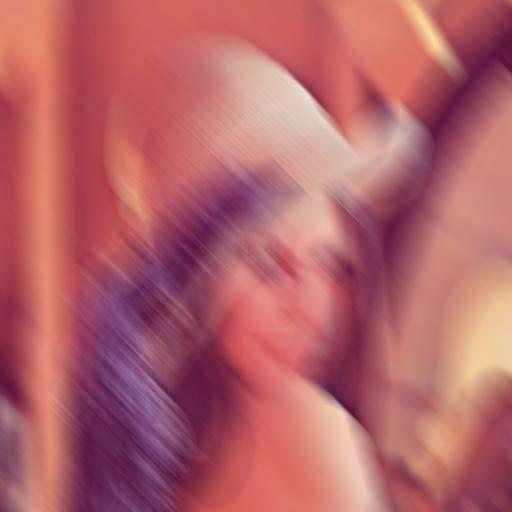
\includegraphics[width=\linewidth]{img/cnn/lena_blur_35x35_45deg.jpg}
        \caption{After a $35\times35$ motion blur filter at 45 degrees (main diagonal)}
    \end{subfigure}
    \vspace{0.3cm}
    \begin{subfigure}[t]{0.49\textwidth}
        \centering
        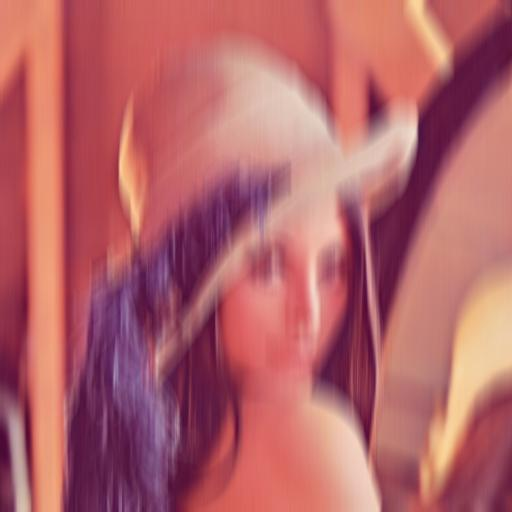
\includegraphics[width=\linewidth]{img/cnn/lena_blur_35x35_90deg.jpg}
        \caption{After a $35\times35$ motion blur filter at 90 degrees (vertical)}
    \end{subfigure}
    \hfill
    \begin{subfigure}[t]{0.49\textwidth}
        \centering
        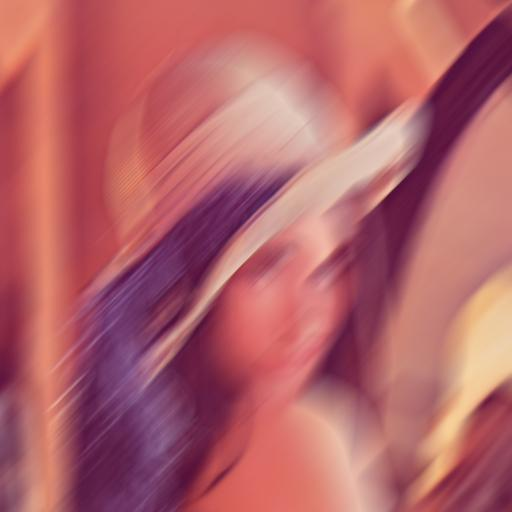
\includegraphics[width=\linewidth]{img/cnn/lena_blur_35x35_135deg.jpg}
        \caption{After a $35\times35$ motion blur filter at 135 degrees (anti-diagonal)}
    \end{subfigure}

    \caption{Effect of a $35\times35$ motion blur filter. Compared to the $9\times9$ filter, the image appears more blurred along the diagonal direction, simulating a longer camera motion during exposure.}
    \label{fig:lena-motion-blur-35x35}
\end{figure}